% \documentclass{book}

\documentclass[12pt]{article}
\usepackage[pdfborder={0 0 0.5 [3 2]}]{hyperref}%
\usepackage[left=1in,right=1in,top=1in,bottom=1in]{geometry}%
\usepackage[shortalphabetic]{amsrefs}%
\usepackage{amsmath}
\usepackage{enumerate}
\usepackage{enumitem}
\usepackage{amssymb}                
\usepackage{amsmath}                
\usepackage{amsfonts}
\usepackage{amsthm}
\usepackage{bbm}
\usepackage[table,xcdraw]{xcolor}
\usepackage{tikz}
\usepackage{float}
\usepackage{svg}
\usepackage{mathtools}
\usepackage{cool}
\usepackage{url}
\usepackage{graphicx,epsfig}
\usepackage{makecell}
\usepackage{array}

\graphicspath{ {images/} }
\renewcommand{\arraystretch}{3}

\begin{document}

\title{}
\author{\vspace{-10ex} }

\begin{center}
{\LARGE APMA 1650 -- Midterm 2}\\
\vspace{5mm}
{\large Thursday, July 28, 2016 }\\
\vspace{10mm}
{\large Name: }
\vspace{3cm}

\begin{figure}[H]
\centering
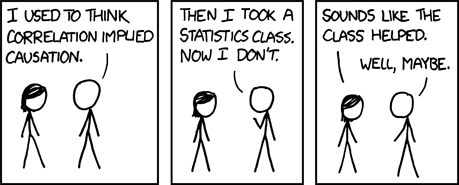
\includegraphics[width=15cm]{correlation}
\end{figure}
% {\large Due Tuesday, July 5, 2016}\\
% \vspace{5mm}
\end{center}
\pagebreak

\begin{center}
{\LARGE Instructions}\\
\vspace{5mm}
\end{center}

\begin{itemize}
\item The exams begins at 1:00 pm and ends at 3:00 pm. You have 2 hours to complete the exam.
\item You may use a calculator if you wish (although the exam is designed to be done without one, so I am not sure how helpful one will be). Other electronic devices may not be used. You may not use any books or notes. 
\item No knowledge of Pok\'emon is required for this exam.
\item Write all answers in the space below the question. If you need more space, feel free to use the back of the page.
\item Correct expressions are sufficient. You do not need to simplify your answers. You can leave answers in terms of binomial coefficients such as $\binom{64}{5}$, exponents such as $(1/2)^{10}$ or $2^{16}$, and factorials such as $12!$.
\item There are 5 questions. Each question is worth 10 points. Partial credit will be given for partially correct answers.
\item Unless you have found an error on the exam, in the interest of fairness, I will likely not answer any questions you have about the test.
\item All answers must be fully justified. Show all of your work. Points will be deducted for unjustified answers.
\item I recommend you look through the entire exam first before answering any questions. That way you can start with the questions you find to be easiest.
\item The list of the common probability distributions, together with their pmfs/densities, expected values, and variances, is included at the back of the exam. A $Z$-table and a $t$-table is also included at the back of the exam.
\end{itemize}

\begin{figure}[H]
\centering
\label{my-label}
\begin{tabular}{|l|l|l|l|l|l|l|}
\hline
Problem & $\:\:1\:\:$ & $\:\:2\:\:$ & $\:\:3\:\:$ & $\:\:4\:\:$ & $\:\:5\:\:$ & Total \\ \hline
Points  &   &   &   &   &   &       \\ \hline
\end{tabular}
\end{figure}

\pagebreak

\begin{enumerate}
\item (10 points) Let $X$ and $Y$ be continuous random variables with joint probability density given by:
\[
f(x,y) = \begin{cases}
cx & x \geq 0, 0 \leq x^2 \leq y \leq 1 \\
0 & \text{otherwise}
\end{cases}
\]
\begin{enumerate}
\item Find the value of $c$ for which $f(x,y)$ is a valid joint probability density function?
\item Find the expected value of $X$.
\item Find the conditional density of $X$ given $Y = y$. Do not forget to include appropriate bounds for the density function.
\end{enumerate}

\pagebreak

\item (10 points) You are interested in the proportion $p$ of registered voters in Pennsylvania who prefer Clinton. You take a sample of $n$ voters from the population. Let $Y$ be the number of voters in your sample who prefer Clinton. We showed in class that $Y \sim \text{Binomial}(n, p)$ and that $\hat{p} = \frac{Y}{n}$ is an unbiased estimator for p. The standard estimator for the variance of $Y$ is:
\[
\hat{V} = n \hat{p}(1 - \hat{p}) = n \left( \frac{Y}{n}\right)\left(1 - \frac{Y}{n} \right)
\]
\begin{enumerate}
\item Show that $\hat{V}$ is a biased estimator for the variance of $Y$.
\item Modify $\hat{V}$ so that you obtain an unbiased estimator for the variance of $Y$.
\end{enumerate}
\pagebreak 

\item (10 points) Suppose you choose a point uniformly at random from the interval $[0, 1]$. After you do so, your friend chooses a point uniformly at random between 0 and your point.
\begin{enumerate}
\item Find the joint probability density function of the two points. Do not forget to include appropriate bounds for the density function.
\item What is the expected value of the product of the two points?
\end{enumerate}

\pagebreak 

\item (10 points) During study breaks from APMA 1650, you play Pok\'emon GO. The average number of Pok\'emon a player catches in a 30-minute period is 6. Assume that Pok\'emon are caught independently from each other.
\begin{enumerate}
\item Suppose you just caught a Pok\'emon. Modeling this with an appropriate probability distribution, what is the probability that it will take less than 10 minutes for you to catch your next Pok\'emon? 
\item Being a good statistician, you decide to play Pok\'emon Go long enough to catch 100 more Pok\'emon. You measure the amount of time it takes to catch each of the 100 Pok\'emon and compute the sample mean. What is the probability that this sample mean is between 4 and 6 minutes?
\end{enumerate}
\pagebreak

\item (10 points) Despite being sleep-deprived from all the Pok\'emon you caught in the previous problem, you decide to continue playing Pok\'emon GO. Once again, the average number of Pok\'emon a player catches in a 30-minute period is 6, and Pok\'emon are caught independently from each other.
\begin{enumerate}
\item Modeling this with an appropriate probability distribution, what is the probability that you catch 1 or fewer Pok\'emon in a 10-minute period?
\item Your friend, who also plays Pok\'emon GO, claims to have caught more than 4 (i.e. 5 or more) Pok\'emon in a 10-minute period. Can you be at least 75\% certain that your friend is lying? Justify your answer mathematically. This does not require a calculator.
\end{enumerate}

\end{enumerate}

\pagebreak 


\begin{figure}[H]
\caption{Discrete Distributions}
\begin{tabular}{l c c c c}
\hline
Distribution & Parameters & Probability Mass Function (pmf) & Mean & Variance \\
\hline
Binomial & $n, p$ & \makecell{ $\displaystyle p(y) = \binom{n}{y}p^y(1-p)^{n-y}$\\$ \displaystyle y = 0, 1, \dots, n$} & $np$ & $np(1-p)$ \\
Geometric & $p$ & \makecell{ $\displaystyle p(y) = (1-p)^{y-1}p$ \\ $y = 1, 2, \dots$} & $ \displaystyle \frac{1}{p}$ & $\displaystyle \frac{1 - p}{p^2}$ \\
Poisson & $\lambda$ & \makecell{ $\displaystyle p(y) = \frac{e^{-\lambda} \lambda^y }{y!}$ \\ $y = 0, 1, 2, \dots$ } & $\lambda$ & $\lambda$ \\
\end{tabular}
\end{figure}

\vspace{2cm}

\begin{figure}[H]
\caption{Continuous Distributions}
\begin{tabular}{l c c c c}
\hline
Distribution & Parameters & Probability Density Function (pdf) & Mean & Variance \\
\hline
Uniform & $a, b$ & \makecell{ $\displaystyle f(y) = \frac{1}{b-a}$ \\ $a \leq y \leq b$ }& $\displaystyle \frac{a + b}{2}$ & $\displaystyle \frac{(b - a)^2}{12}$ \\
Exponential & $\lambda$ & \makecell{ $\displaystyle f(y) = \lambda e^{-\lambda y}$ \\ $0 \leq y < \infty$} & $\displaystyle \frac{1}{\lambda}$ & $\displaystyle \frac{1}{\lambda^2}$ \\
Normal & $\mu, \sigma$ & $\displaystyle f(y) = \frac{1}{\sqrt{2 \pi}\sigma}e^{- \frac{(y - \mu)^2}{2 \sigma^2}}$ & $\mu$ & $\sigma^2$ \\
Standard Normal & none & $\displaystyle f(y) = \frac{1}{\sqrt{2 \pi}}e^{- \frac{y^2}{2}}$ & $0$ & $1$ \\
\end{tabular}
\end{figure}

\end{document}

